\begin{figure}[t]
\centering

\begin{subfigure}[b]{0.49\columnwidth}
\centering 
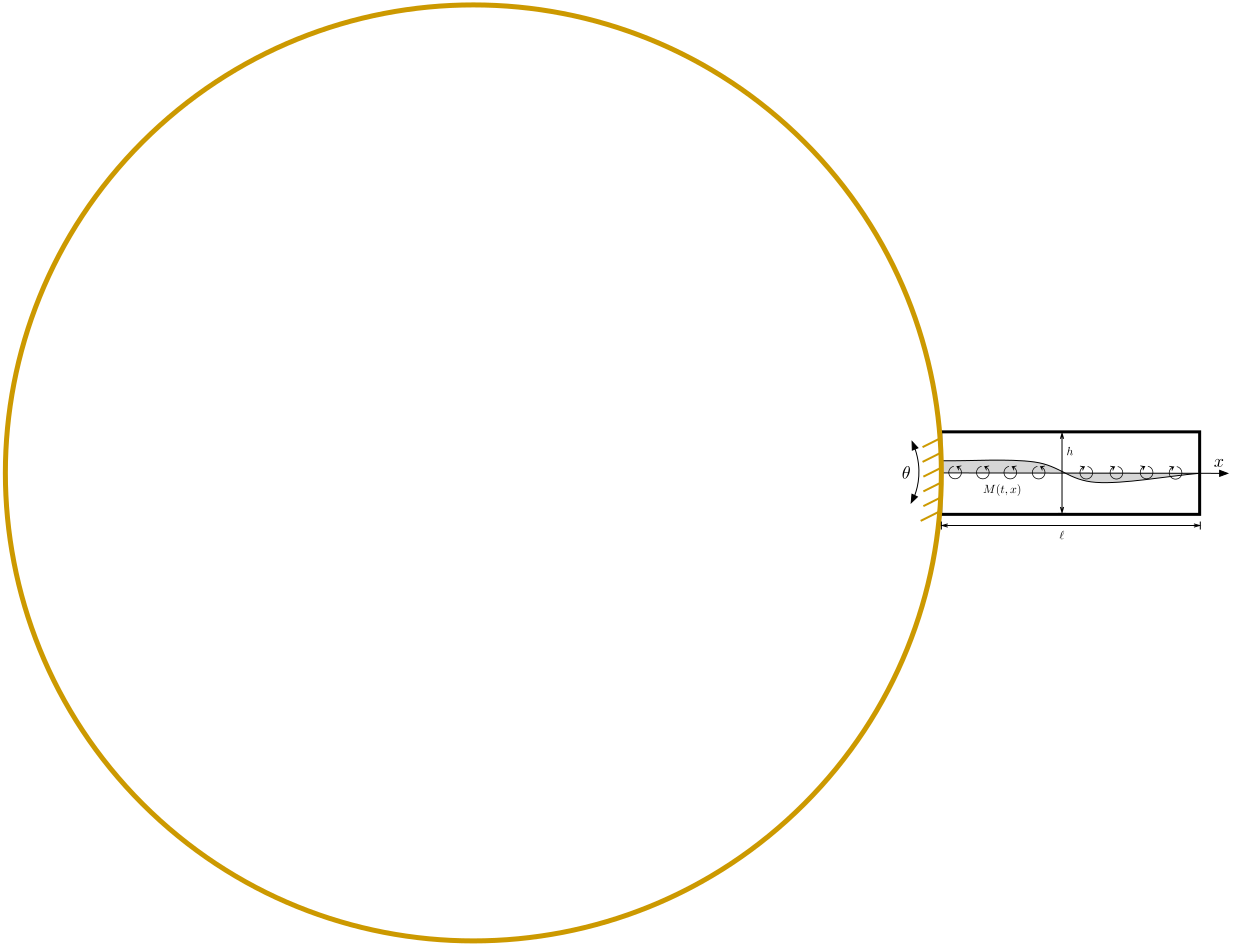
\includegraphics[width=\columnwidth,trim=12.46in 5.3in 0in 5.44in,clip=true]{../ch7/figures/varbeam-c-ut-2}
\caption{Continuously distributed internal moment on a uniform thickness array.}\label{fig:ch7:varbeam-c-ut}
\end{subfigure}
\hspace{0.005\columnwidth}
\begin{subfigure}[b]{0.49\columnwidth}
\centering 
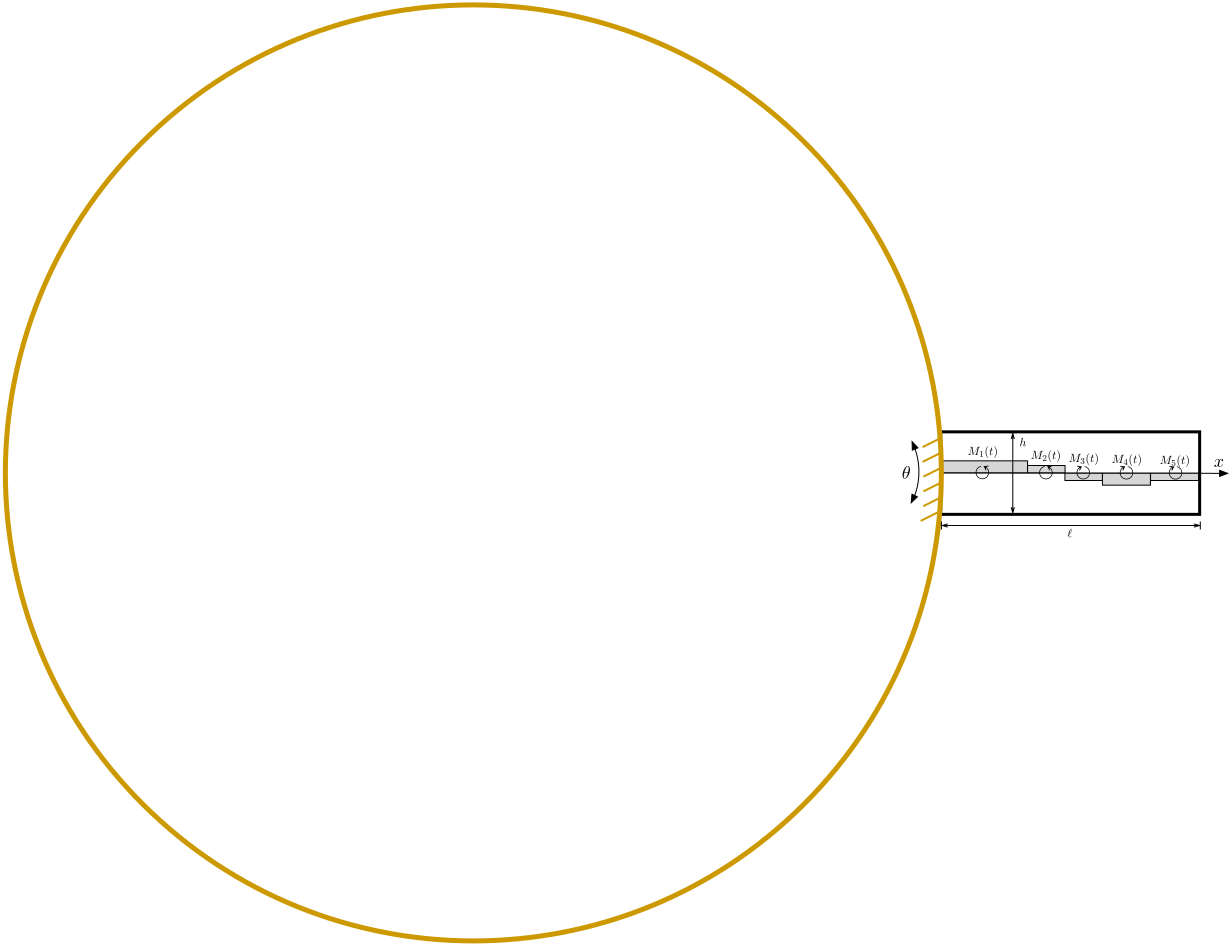
\includegraphics[width=\columnwidth,trim=12.46in 5.3in 0in 5.44in,clip=true]{../ch7/figures/varbeam-d-ut-2}
\caption{Piecewise constant distributed internal moment on a uniform thickness array.}\label{fig:ch7:varbeam-d-ut}
\end{subfigure}%

\begin{subfigure}[b]{0.52\columnwidth}
\centering 
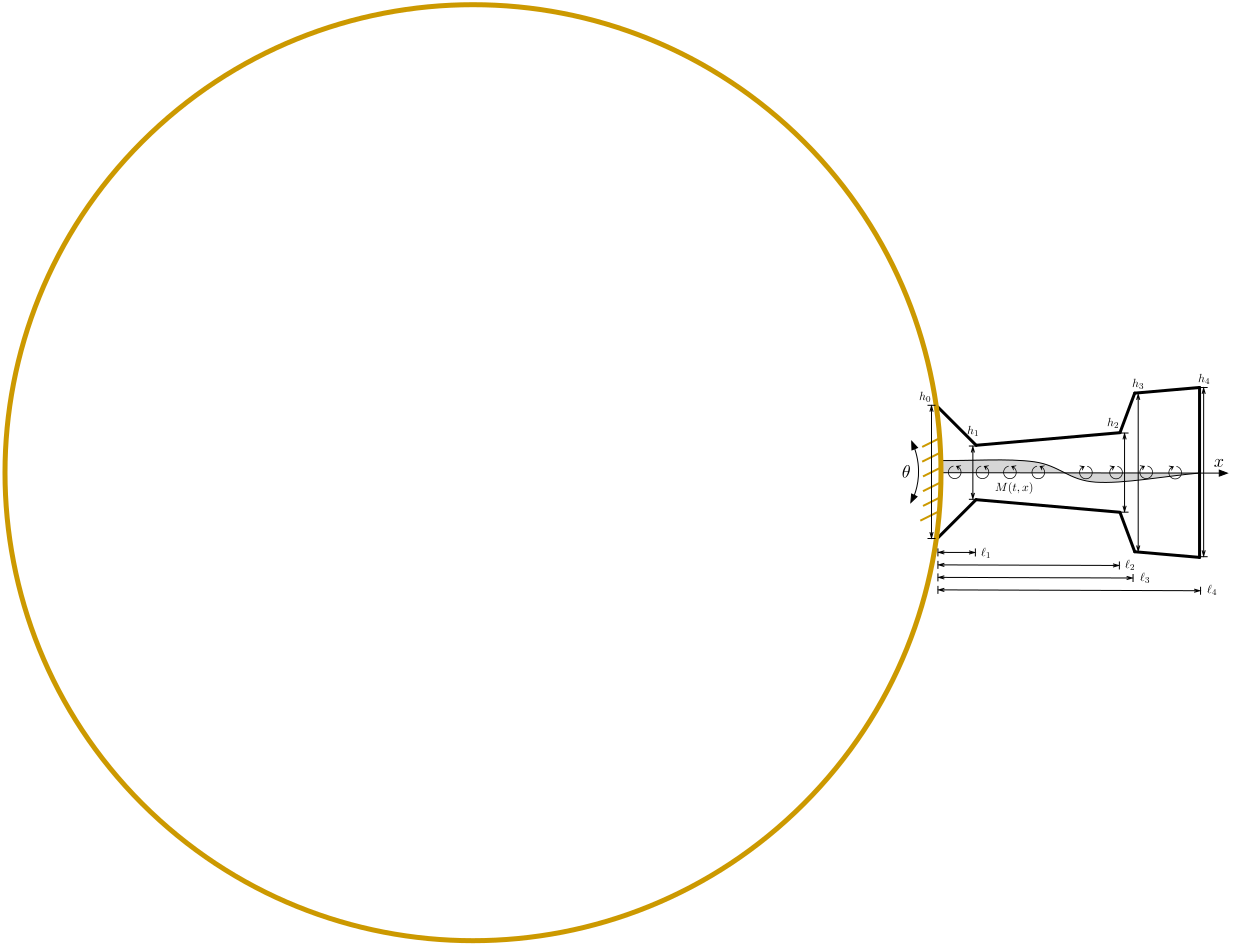
\includegraphics[width=\columnwidth,trim=12.46in 4.8in 0in 5.1in,clip=true]{../ch7/figures/varbeam-c-vt-2}
\caption{Piecewise linear distributed array thickness.}\label{fig:ch7:varbeam-c-vt}
\end{subfigure}%

\caption{Illustrations of various design representations for internally actuated array design problems for pointing. \label{fig:ch7:varbeam}}
\end{figure}